\documentclass[11pt,a4paper]{article}
\usepackage[utf8]{inputenc}
\usepackage[T1]{fontenc}
\usepackage[polish]{babel}
\usepackage{lmodern}
\usepackage{graphicx}
\usepackage{epstopdf}
\usepackage{anysize}
\usepackage{makeidx}
\usepackage{hyperref}



\makeatletter
\renewcommand{\maketitle}{
\begin{titlepage}
\begin{center}

\LARGE{AKADEMIA GÓRNICZO-HUTNICZA}

\vspace*{1cm}

\includegraphics[scale=1.8]{agh.eps}
\vspace*{1cm}

\LARGE{im. Stanisława Staszica w Krakowie}

\rule{\textwidth}{0.4mm}
\LARGE \textsc{\@title}
\rule{\textwidth}{0.4mm}

\vspace*{5mm}


\large
\emph{Autorzy:}\\
Bartłomiej \textsc{Bułat}\\
Tomasz \textsc{Czarnik}\\
Krzysztof \textsc{Śmiłek}\\

\vfill
\vspace*{\stretch{8}}
\rule{\textwidth}{0.4mm}

\large{Wydział Elektroniki, Automatyki, Informatyki i Elektrotechniki}\\
\large{Katedra Automatyki}\\
\large{Laboratorium Biocybernetyki}\\
\vspace*{\stretch{7}}
\@date

\end{center}

\end{titlepage}
}
\makeatother

\title{Badanie metod rozpoznawania\\twarzy na obrazach}
\date{\today}

\makeindex

\begin{document}

\maketitle

\newpage

\tableofcontents

\newpage

\section{Wstep}

\subsection{Problem rozpoznawania twarzy i ogólny algorytm}

Rozpoznanie twarzy na obrazie nie jest trywialnym problemem. Składa się ono z kilku etapów o różnej złożoności. Na złożoność zadania wpływa to, że trudne jest uzyskanie zdjęcia twarzy na jednolitym tle i zawsze w tej samej pozycji. Czasami do akwizycji obrazu twarzy stosuje się inne metody niż normlane zdjęce 2D. Często wykorzystywane metody to obrazy termowizyjne dostarczajęce dodatkowych informacji o rozkładzie temperatur na twarzy oraz metody operujące na obrazach 3D, uzyskanych zapomocą stereowizji lub specjalnych skanerów. Po akwizycji obraz następuje etap wyszukiwania wzorców które są kandydatami na bycie twarzą. Najprostrze metody to te bazujące na kolorze twarzy. Innymi metodami są metody statystyczne jak również sieci neuronowe (które wykorzystywane są nie tylko do lokalizacji, ale i do klasyfikacji twarzy). Wykryte obiekty są następne klasyfikowane poprzez porównywanie wektorów cech wyliczonych ze znalezionych obiektów. Głowne metody ekstrakcji cech to metody strukturalne (opis lokalnych cech twarzy tj. oczy, usta czy nos za pomocą współrzednych czy parametrów statystycznych) oraz metody całościowe gdzie cała twarz dostarcza danych do analizy np. PCA.

\section{Metody Rozpoznawania Twarzy}

\subsection{Metody geometryczne}
W metodach tych twarz charakteryzowana jest przez zbiór wartości kątów, odległości czy też pól wyznaczonych w oparciu o charakterystyczne punkty, takie jak środki oczu, koniec nosa itd. Problemem jest tutaj precyzyjne zlokalizowanie odpowiednich fragmentów twarzy. Staje się to szczególnie trudne gdy zdjęcie poddane analizie nie jest wykonane bezpośrednio od przodu, gdyż wówczas niektóre istotne części twarzy mogą być nawet całkowicie niewidoczne. Sporządzanie opisu matematycznego poprzez wyznaczenie geometrycznych parametrów było jednym z pierwszych, najbardziej intuicyjnych pomysłów na ekstrakcję cech w rozpoznawaniu twarzy. Obecnie jednak podejście to praktycznie nie jest już rozwijane, gdyż istnieją mechanizmy wykrywające twarze szybciej oraz z większą skutecznością.

\subsection{Metoda analizy kolorów}
W metodzie tej na podstawie odpowiednich schematów kolorów wykrywa się wszystkie elementy na obrazie zgodne z danym schematem. Niestety metoda ta jest bardzo wrażliwa ponieważ poza twarzą wykrywa też dłonie, szyję itp. Dlatego też dodatkowo zwykle należy przeprowadzić po niej selekcję po kształcie i rozmiarze wykrytych regionów. 
\\
\\
\noindent Zalety:
\begin{itemize}
\item szybkość
\item brak ograniczeń odnośnie orientacji oraz rozmiaru twarzy
\end{itemize}

\noindent Wady:
\begin{itemize}
\item baza schematów kolorów jest ograniczona
\item duża podatność metody na natężenie jasności zdjęcia
\item obiekty o kolorze podobnym do koloru skóry są także wykrywane
\end{itemize}

\subsection{Metoda Sieci neuronowych}
Operację wykrywania twarzy za pomocą tego systemu można podzielić na 3 główne składowe:
\begin{enumerate}
\item Inicjalizacja (projektowanie i tworzenie sieci neuronowych)
\item Trening (wybór danych do trenowania, wybór cech, właściwe trenowanie)
\item Klasyfikacja (skanowanie obrazów w celu zlokalizowania twarzy)
\end{enumerate}

\noindent 
Do tego celu tworzone są jednokierunkowe warstwowe sieci neuronowe, które są trenowane przy użyciu metody wstecznej propagacji. Dane treningowe zawierają obrazy z twarzami lub bez. Przepuszczając przez sieć wybrany obraz, równocześnie na wyjściu z sieci ustalamy ostateczny wynik (1 – twarz, -1 – obraz bez twarzy).  Dzięki wspomnianej wcześniej metody wstecznej propagacji, na podstawie wyjścia z całej sieci, komórki wewnętrzne są w stanie same kalibrować swoje wartości tak, aby sprostać wymogom całej sieci.\\
Poddając dany obraz badaniu na obecność twarzy, jest on skalowany i dzielony na okna, które są indywidualnie przepuszczane przez sieć. Okna, które zawierają twarze są otaczane obwiednią, następnie wszystkie okna są łączone ponownie w całość i następuje skalowanie obrazu do pierwotnego rozmiaru. Dzięki temu na obrazie końcowym możemy ujrzeć przeskalowane prostokąty, które wskazują, w którym konkretnie miejscu znaleziono twarze.

\vspace*{1cm}
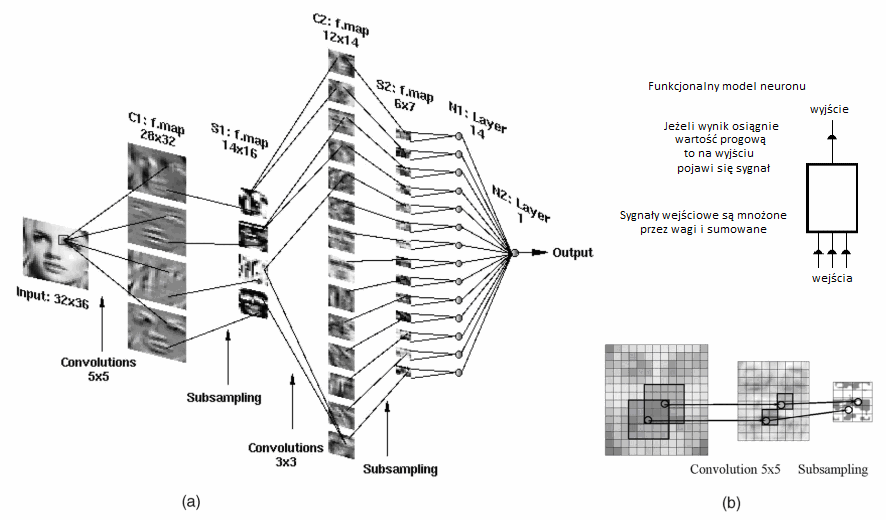
\includegraphics[scale=0.65]{cnn.png}
\vspace*{1cm}

\noindent 
Zalety:
\begin{itemize}
\item  Bardzo dobre rozpoznawanie wzorców
\item  Praca z zaszumianymi i niepełnymi danymi
\item  Możliwość pracy równoległa z wielu wejść
\item  Rozwiązanie problemu bez jego dogłębnej analizy
\item  Duża tolerancja na błędy
\end{itemize}

\noindent 
Wady:
\begin{itemize}
\item  Długi czas uczenia 
\item  Sukces uczenia nie jest gwarantowany 
\item  Problemy z wyborem danych do treningu sieci 
\end{itemize}

\subsection{Model aktywnego kształtu}
Tim Cootes i Chris Taylor w roku 1995 opracowali metodę modelu aktywnego kształtu (Active Shape Model). Jest to model statyczny, w którym jego kształt poprzez dozwolone deformacje próbuje się automatycznie dopasowywać do obiektu znajdującego się na obrazie. Określa się wzorzec obiektu jako model rozkładu punktów (Point Distribution Model), czyli zbiór etykietowanych punktów określających poszukiwany kształt. Następnie przeprowadzany jest proces uczenia w którym zbiera się informacje o różnych modyfikacjach wzorca. W tym celu przeważnie na kolejne zdjęcia testowe twarzy nanosi są ręcznie punkty charakterystyczne. Otrzymane wektory punktów poddaje się procesowi normalizacji (taki model będzie można dowolnie przeskalowywać, zachowana jest jedynie informacja o kształcie). Na koniec należy obliczyć kształt średni, odchylenie od średniej dla każdego elementu zbioru uczącego oraz obliczyć wektory własne odpowiedniej macierzy kowariancji. Konstruuje się model utworzony z średniego kształtu i sumy ważonej najbardziej charakterystycznych deformacji. Algorytm pozwala na deformację kształtu średniego tylko w ograniczonym zakresie.\\
\\
\noindent
Lista kroków algorytmu wyszukiwania obiektu:
\begin{itemize}
\item badane jest sąsiedztwo każdego punktu charakterystycznego w poszukiwaniu odpowiedniej deformacji
\item obliczane są optymalne parametry przesunięcia, obrotu, skali tak aby umieścić niezdeformowany model jak najbliżej rzeczywistego kształtu
\item uważając na dopuszczalny zakres zmian uaktualnia się parametry modelu dopasowując go jak najdokładniej do obrazu
\end{itemize}

Przesunięcie punktów charakterystycznych określa się na podstawie odnalezionych krawędzi znajdujących się na linii prostopadłej do brzegu modelu. Dysponując informacją o poziomach jasności wokół punktów modelu można też próbować odnajdywać miejsca w sąsiedztwie dla którego profil jasności najbardziej przypomina ten z modelu. \\

\noindent 
Zalety:
\begin{itemize}
\item duża elastyczność - model potrafi dopasować się do różnych kształtów
\item uniwersalny - kształt określany jest w drodze uczenia
\item pomocny przy klasyfikowaniu i identyfikowaniu twarzy
\end{itemize}

\noindent 
Wady:
\begin{itemize}
\item  czasochłonne i trudne uczenie modelu 
\item  mało odporny na zmieniające się warunki oświetlenia, zróżnicowanego tła, bardziej realistycznych warunków
\item  słabe wyniki dla osób z długimi ciemnymi włosami
\end{itemize}

\section{Podsumowanie}

\section{Bibliografia}

\bibliography{bibliography}

\end{document}
